\documentclass[a4paper, oneside, openany, dvipsnames, table, 12pt]{article}
\usepackage{../Template/AFKstyle}
\usepackage{hyperref}
\usepackage{amsmath}
\newcommand{\Titolo}{Verbale interno 2020-06-05}

\newcommand{\Gruppo}{TeamAFK}

\newcommand{\Redattori}{}

\newcommand{\Verificatori}{}

\newcommand{\pathimg}{../../../../Template/img/logoAFK.png}

\newcommand{\Approvatore}{}

\newcommand{\Distribuzione}{Prof. Vardanega Tullio \newline Prof. Cardin Riccardo \newline TeamAFK}

\newcommand{\Uso}{Interno}

\newcommand{\NomeProgetto}{"Predire in Grafana"}

\newcommand{\Mail}{gruppoafk15@gmail.com}

\newcommand{\Versionedoc}{1.0.0}

\newcommand{\DescrizioneDoc}{Riassunto dell'incontro del gruppo \textit{TeamAFK} tenutosi il 2020-06-05.}


\makeindex

\begin{document}
\copertina{}

%------------------ COLORI TABELLE 
\definecolor{pari}{RGB}{255, 207, 158} %{HTML}{E1F5FE} %azzurrino
\definecolor{dispari}{HTML}{FAFAFA} %bianco/grigetto 

%definizione colori per tabelle (tranne copertina)
\definecolor{redafk}{RGB}{255, 133, 51}
\definecolor{grey2}{RGB}{204, 204, 204}
\definecolor{greyRowafk}{RGB}{234, 234, 234}
\definecolor{lastrowcolor}{RGB}{176, 196, 222} %steel blue %{255,165,0} orange %{RGB}{255, 207, 158}
\rowcolors{2}{pari}{dispari}
\renewcommand{\arraystretch}{1.5}

%------------------

\newpage
\section*{Registro delle modifiche}
{
	\centering
	\begin{longtable}{ c c  C{4cm}  C{4cm}  C{3cm} }
		\rowcolor{redafk}
		\textcolor{white}{\textbf{Versione}} & \textcolor{white}{\textbf{Data}} & \textcolor{white}{\textbf{Descrizione}} & \textcolor{white}{\textbf{Nominativo}} & \textcolor{white}{\textbf{Ruolo}}\\		
		2.1.1 & 2020-05-27 & Aggiunta incrementi \S 6.2. Verificato il documento. & &\adm{} \newline \ver{} \\
		2.1.0 & 2020-05-26 & Refactoring \S 4.1 e \S 4.3. Apportate modifiche normative al \textit{Registro delle Modifiche}. Verificato il documento. & Davide Zilio \newline Victor Dutca & \adm{} \newline \ver{} \\
		2.0.0 & 2020-05-10 & Approvazione del documento per la RP. & Davide Zilio &\RdP{} \\
		1.1.0 & 2020-05-08 & Stesura \S 6.2. Verificato il documento. & Simone Meneghin \newline Alessandro Canesso &\adm{} \newline \ver{}\\
		1.0.2 & 2020-05-06 & Ampliamento \S 2. Verificato il documento. & Victor Dutca \newline Alessandro Canesso &\Res{} \newline \ver{}\\
		1.0.1 & 2020-04-30 & Correzioni e stesura \S 2.1. Verificato il documento. & Simone Meneghin \newline Alessandro Canesso &\Res{} \newline \ver{}\\
		1.0.0 & 2020-04-12 & Approvazione del documento per la RR. & Victor Dutca &\RdP{} \\
		0.7.0 & 2020-03-10 & Stesura \S B. Verificato il documento. & Alessandro Canesso \newline Olivier Utshudi &\Res{} \newline \ver{}\\
		0.6.0 & 2020-03-10 & Stesura \S 6. Verificato il documento. & Alessandro Canesso \newline Olivier Utshudi &\Res{} \newline \ver{}\\
		0.5.0 & 2020-03-06 & Stesura \S 5. Verificato il documento.  & Fouad Farid \newline Olivier Utshudi &\Res{} \newline \ver{}\\
		0.4.0 & 2020-04-04 & Stesura \S 4. Verificato il documento. & Simone Federico Bergamin \newline Simone Meneghin &\adm{} \newline \ver{}\\	
		0.3.0 & 2020-04-03 & Stesura \S 3. Verificato il documento.  & Simone Federico Bergamin \newline Olivier Utshudi &\adm{} \newline \ver{}\\	
		0.2.0 & 2020-03-30 & Stesura \S 2. Verificato il documento.  & Alessandro Canesso \newline Simone Meneghin &\Res{} \newline \ver{}\\	
		0.1.0 & 2020-03-30 & Stesura \S 1. Verificato il documento. & Alessandro Canesso \newline Simone Meneghin &\Res{} \newline \ver{}\\		
	\end{longtable}
} 


%Didascalia tabelle/immagini (prendono come riferimento la subsection)
\counterwithin{table}{subsection}
\counterwithin{figure}{subsection}
\newpage

%indice, indice figure e indice tabelle
\tableofcontents
\newpage
\listoffigures
\newpage
\listoftables
\newpage

\section{Introduzione}

\subsection{Scopo del documento}
Il seguente documento ha il compito di stabilire le regole che il team di sviluppo intende seguire in ogni attività di progetto, così da omologare il materiale prodotto.
I fornitori intendono adottare un approccio incrementale\glo, affinché lo sviluppo del prodotto si basi su decisioni prese di comune accordo. Perciò ogni componente del team deve far riferimento a questo documento per garantire la coesione e uniformità delle scelte prese.

\subsection{Scopo del prodotto}
Il capitolato {C4}\glo illustra il prodotto da fornire. Tale prodotto consiste in tool di addestramento ed un plugin\glo di Grafana\glo che prenderà il nome \textit{Predire in Grafana}. Entrambi gli applicativi verranno scritti in linguaggio JavaScript\glo. Il primo avrà il compito di produrre un file di estensione JSON\glo basato su dati di addestramento\glo. Il secondo invece si occuperà di leggere il file creato, effettuare previsioni basandosi su di esso e rendere disponibili al sistema i risultati ottenuti, in modo da poterli visualizzare in grafici e dashboard.
\subsection{Glossario}
Per evitare ambiguità nei documenti formali, viene fornito il documento \textit{Glossario\_v2.0.0}, contenente tutti i termini considerati di difficile comprensione. Perciò nella documentazione fornita ogni vocabolo contenuto in \textit{Glossario\_v2.0.0} è contrassegnato dalla lettera \textit{G} a pedice.
\subsection{Riferimenti}
\subsubsection{Riferimenti normativi}
\begin{itemize}
	\item \textbf{Capitolato d'appalto C4 - Predire in Grafana}: \\
	\url{https://www.math.unipd.it/~tullio/IS-1/2019/Progetto/C4.pdf}.	
\end{itemize}
\subsubsection{Riferimenti informativi}
\begin{itemize}
	\item \textbf{Change Management Process}: \\
	\href{https://www.blog-management.it/2018/04/10/change-management-project-management/}{https://www.blog-management.it/change-management-project-management}\\
	\href{https://www.digital4.biz/hr/hr-transformation/digital-transformation-e-change-management-vanno-avanti-di-pari-passo/}{https://www.digital4.biz/hr/hr-transformation/};
	\item \textbf{The three P's of Software Engineering}: \\
	\url{http://dwaynephillips.net/CutterPapers/ppp/ppp.htm}
	\item \textbf{Software Engineering - Ian Sommerville - 10th Edition}
	\item \textbf{Slide L05 del corso Ingegneria del Software - Ciclo di vita del software}: \\
	\url{https://www.math.unipd.it/~tullio/IS-1/2019/Dispense/L05.pdf};
	\item \textbf{Slide L06 del corso Ingegneria del Software - Gestione di Progetto}: \\
	\url{https://www.math.unipd.it/~tullio/IS-1/2019/Dispense/L06.pdf};	
	\item \textbf{Slide L12 del corso Ingegneria del Software - Qualità di Prodotto}: \\
	\url{https://www.math.unipd.it/~tullio/IS-1/2019/Dispense/L12.pdf};
	\item \textbf{Slide L13 del corso Ingegneria del Software - Qualità di Processo}: \\
	\url{https://www.math.unipd.it/~tullio/IS-1/2019/Dispense/L13.pdf};
\end{itemize}
\pagebreak

\section{Processi primari}
	\subsection{Fornitura}
		\subsubsection{Scopo}
		Lo scopo del processo di fornitura consiste nelle attività e compiti dell'acquirente, come risposta ai bisogni del cliente in ambito di sistema, prodotto e/o servizio software. Nello specifico, le caratteristiche richieste dal proponente sono analizzate e stilate nello \textit{Studio di Fattibilità}, il quale è alla base del processo di fornitura. Dopodiché è possibile stabilire le risorse e le procedure necessarie alla redazione di un \textit{Piano di Progetto} da seguire fino alla consegna del materiale prodotto.
		Nel dettaglio le attività svolte da questo processo sono:
		\begin{itemize}
			\item avvio;
			\item studio di fattibilità;
			\item contrattazione;
			\item progettazione;
			\item esecuzione e controllo;
			\item revisione e valutazione;
			\item consegna e completamento.
		\end{itemize}
		\subsubsection{Aspettative}
		Il gruppo deve avere un frequente contatto con il cliente al fine di rispettare i vincoli obbligatori da lui fissati, onde evitare di scostarsi troppo dal prodotto finale richiesto. Per questo è necessario comunicare con il proponente, per poter aver chiari i bisogni che tale prodotto intende soddisfare con le sue funzionalità. Quindi, ogniqualvolta il gruppo venga a contatto con il proponente, deve stabilire:
		\begin{itemize}
			\item aspetti chiave che soddisfano i bisogni richiesti;
			\item requisiti e vincoli dei processi;
			\item verifica continua;
			\item chiarimento di eventuali dubbi;
			\item accordo sulla qualifica del prodotto.
			\end{itemize} 
		\subsubsection{Descrizione}
		Questa sezione ha il compito mostrare le norme che \textit{TeamAFK} adotterà in tutte le attività di progettazione, sviluppo e consegna del prodotto \textit{Predire in Grafana}, con lo scopo di diventare fornitori del capitolato proposto dalla proponente \textit{Zucchetti SPA} e dai committenti Prof. Tullio Vardanega e Prof. Riccardo Cardin.
		\subsubsection{Attività}
			\paragraph{Avvio}
			\paragraph*{Studio di Fattibilità} \mbox{} \\ \mbox{} \\
			Lo \textit{Studio di Fattibilità}, redatto per ogni capitolato\glo dagli analisti, illustra:
			\begin{itemize}
				\item \textbf{Descrizione generale}: sintesi delle informazioni generali del capitolato e delle circostanze da cui sorgono tali richieste;
				\item \textbf{Obiettivi}: vengono mostrate le caratteristiche principali del prodotto ed i relativi obiettivi da raggiungere;
				\item \textbf{Tecnologie utilizzate}: corrisponde all'elenco degli strumenti messi a disposizione dall'azienda proponente al team per sviluppare il progetto;
				\item \textbf{Valutazione finale}: si tratta di un commento elaborato dal gruppo una volta riunitosi e analizzato le  richieste dell'azienda, motivando la scelta di focalizzarsi o meno su una determinata offerta.
			\end{itemize}
			\paragraph{Contrattazione} \mbox{} \\ \mbox{} \\
			L'attività di contrattazione prevede la discussione dei termini di sviluppo del progetto sia per quanto concerne l'aspetto economico, sia per quanto riguarda l'aspetto dei requisiti che il prodotto finale deve rispettare. Come base di discussione il \textit{TeamAFK} propone il preventivo all'interno del \textit{Piano di Progetto} e la lista dei requisiti esposti all'interno dell'\textit{Analisi dei Requisiti}. Il gruppo si impegna ad aggiornare tali
valutazioni proposte sulla base dei feedback e della discussione con il committente.
			\paragraph{Progettazione} \mbox{} \\ \mbox{} \\
			L'attività di progettazione prevede la redazione di un \textit{Piano di Progetto} che definisca le linee guida per la gestione e la realizzazione del progetto e che garantisca il raggiungimento degli obiettivi entro i termini prefissati.	
			
			\paragraph*{Coinvolgimento di committente e proponente}	\mbox{} \\ \mbox{} \\
			Il \textit{TeamAFK} prevede di coinvolgere il proponente Gregorio Piccoli - \textit{Zucchetti SpA} nell'analisi dei requisiti e nello sviluppo del progetto tramite incontri su appuntamento. Il coinvolgimento del committente è invece garantito dalla presenza di revisioni periodiche, come previsto dalle regole di progetto.		
			
			\paragraph*{Piano di Progetto} \mbox{} \\ \mbox{} \\
			Il \textit{Piano di Progetto} è un documento redatto dal progect manager\glo e dagli amministratori; si aggiunge all'insieme dei documenti che il team dovrà seguire per tutta la durata del progetto. In particolare questo documento conterrà:
			\begin{itemize}
				\item \textbf{Analisi dei rischi}: il fornitore analizza tutti gli eventuali rischi di tipo tecnico, economico e temporale che possono presentarsi durante il progetto, fornendo anche soluzioni che possano risolverli o almeno limitare i loro effetti negativi;
				\item \textbf{Modello di sviluppo}: viene definita la struttura su cui basarsi per la pianificazione, esecuzine e consegna del prodotto software;
				\item \textbf{Pianificazione}: viene pianificato l'insieme delle attività da seguire durante le fasi di progetto, collocandole nel tempo e stabilendo le loro scadenze;
				\item \textbf{Preventivo e consuntivo}: con il preventivo viene mostrata una stima di quello che sarà il carico di lavoro che il team sosterrà durante il progetto, in termini di tempo e i relativi costi. Con il consuntivo di periodo, invece verranno riportati le variazioni dei costi rispetto a quanto preventivato.
			\end{itemize}
			\paragraph{Esecuzione e controllo} \mbox{} \\ \mbox{} \\
Il fornitore deve attuare ed eseguire i piani sviluppati nella fase di pianificazione e sviluppare il prodotto software monitorando il progresso e la qualità.
			\paragraph*{Piano di Qualifica} \mbox{} \\ \mbox{} \\
			I verificatori si occuperanno di redigere il \textit{Piano di Qualifica}, ovvero l'insieme di attività con il compito di fissare obiettivi di qualità del prodotto nel suo complesso. Verranno quindi considerati anche i processi e le risorse necessarie a raggiungere tali obiettivi. Nel dettaglio il \textit{Piano di Qualifica} si focalizza su:
			\begin{itemize}
				\item \textbf{Qualità di prodotto}: vengono fissate le politiche per il raggiungimento della qualità, gli obiettivi da raggiungere e gli strumenti necessari al controllo;
				\item \textbf{Qualità di processo}: stabilire sulla base di opportune misurazioni il grado di efficacia ed efficienza di un processo a partire dalla sua definizione;
				\item \textbf{Valutazione di miglioramento}: i problemi e le relative soluzioni vengono evidenziate in questa sezione del \textit{Piano di Qualifica};
				\item \textbf{Resoconto dell'attività di verifica}: vengono riportate i risultati delle metriche come resoconto dell'attività di qualifica.
			\end{itemize}
			
			\paragraph*{Standard di Qualità} \mbox{} \\ \mbox{} \\
			La sezione \S A descrive gli standard di qualità seguiti per lo sviluppo della qualità del progetto.
			
			\paragraph{Revisione e valutazione} \mbox{} \\ \mbox{} \\
			Il fornitore deve eseguire la verifica e validazione al fine di dimostrare che il prodotto software soddisfi i requisiti descritti nell' \textbf{Analisi dei Requisiti}.
			\paragraph{Consegna e completamento} \mbox{} \\ \mbox{} \\		
			Il fornitore consegna il prodotto software come specificato dal contratto.
		\subsubsection{Strumenti}
		Di seguito sono illustrati gli strumenti utilizzati per lo svolgimento dell'attività di fornitura.
		\begin{itemize}
			\item \textbf{GanttProject}: software per la produzione di diagrammi di Gantt\glo (analizzato nel dettaglio in § 3.8.3);
			\item \textbf{Google Calendar}: sistema di calendari gestito da Google.
		\end{itemize}

	\subsection{Sviluppo}
		\subsubsection{Scopo}È il processo che si occupa di stabilire le attività da svolgere per costruire e consegnare il prodotto finale.
		\subsubsection{Aspettative}
		Le aspettative sono le seguenti:
			\begin{itemize}
				\item stabilire obiettivi di sviluppo;
				\item stabilire vincoli tecnici;
				\item stabilire vincoli di design;
				\item realizzare il prodotto software che superi i test, e soddisfi i vincoli di progetto.
			\end{itemize}
		\subsubsection{Descrizione}
			Il processo di sviluppo si divide in:
				\begin{itemize}
					\item \textit{Analisi dei Requisiti};
					\item Progettazione;
					\item Codifica.
				\end{itemize}
		\subsubsection{Attività}
			\paragraph{Analisi dei Requisiti} \mbox{} \\ \mbox{} \\
			L'elenco dei requisiti necessari allo svolgimento del processo di sviluppo viene raccolto e redatto dagli analisti in un apposito documento di \textit{Analisi dei Requisiti}. Quest'ultimo ha lo scopo di:
				\begin{itemize}
					\item descrivere l'obiettivo del prodotto;
					\item fornire ai progettisti riferimenti precisi ed affidabili;
					\item stabilire le prospettive e le funzionalità del prodotto in base ai vincoli fissati dal proponente;
					\item fornire ai verificatori riferimenti affidabili per la loro attività di controllo;
					\item valutare rischi, costi e benefici in relazione al carico di lavoro.
				\end{itemize} 
			\subparagraph*{Aspettative} \mbox{} \\ \mbox{} \\
			L'obiettivo di questa attività è quello di redigere un documento formale contenente tutti i requisiti richiesti dal progetto.
			\subparagraph*{Descrizione} \mbox{} \\ \mbox{} \\
			I requisiti saranno raccolti nel seguente modo:
				\begin{itemize} 
					\item lettura del capitolato d'appalto;
					\item confronto con il proponente;
					\item discussione tra i componenti del gruppo;
					\item studio dei casi d'uso.
				\end{itemize}
				\subparagraph*{Casi d'uso} \mbox{} \\ \mbox{} \\
				I casi d'uso sono scenari che descrivono una possibile sequenza di iterazioni dell'utente, visto come attore\glo attivo e/o passivo, e il sistema. La struttura di un caso d'uso è la seguente:
				\begin{itemize}
					\item codice identificativo;
					\item titolo;
					\item diagramma UML\glo (se presente);
					\item attore primario;
					\item precondizioni;
					\item postcondizioni;
					\item scenario principale;
					\item inclusioni (se presenti);
					\item estensioni (se presenti).

				\end{itemize}
				\subparagraph*{Codice identificativo dei casi d'uso} \mbox{} \\ \mbox{} \\
			Il codice di ogni caso d'uso seguirà questo formalismo: \\ \\
			\centerline{\textbf{UC[codice\_padre].[codice\_figlio]}} \\ \\
			\textbf{Requisiti} \\ \\
			I requisiti seguiranno la seguente struttura:
				\begin{itemize}
					\item \textbf{codice identificativo}: è un codice univoco e conforme alla codifica: \\ \\
					\centerline{\textbf{Re[Importanza][Tipologia][Codice]}} \\ \\
					Le voci riportate nella precedente codifica significano: 
					\begin{itemize}
						\item \textbf{Importanza}: la quale può assumere come valori:
						\begin{itemize}
							\item 1: requisito obbligatorio, irrinunciabile;
							\item 2: requisito desiderabile, perciò non obbligatorio ma riconoscibile;
							\item 3: requisito opzionale, ovvero trattabile in un secondo momento o relativamente utile.
						\end{itemize}
						\item \textbf{Tipologia}: la quale può assumere come valori:
						\begin{itemize}
							\item F: requisito funzionale;
							\item P: requisito prestazionale;
							\item Q: requisito di qualità;
							\item V: requisito di vincolo.
						\end{itemize}
						\item \textbf{Codice identificativo}: il quale è un identificatore univoco del requisito, e viene espresso in forma gerarchica padre/figlio.
					\end{itemize}
					\item \textbf{Classificazione}: specifica il peso del requisito facilitando la sua lettura anche se causa ridondanza;
					\item \textbf{Descrizione}: sintesi completa di un requisito;
					\item \textbf{Fonti}: il requisito può avere le seguenti provenienze:
					\begin{itemize}
						\item capitolato;
						\item interno: requisito che gli analisti ritengono di aggiungere in base alle esigenze del team;
						\item caso d'uso: il requisito proviene da uno o più casi d'uso, dei quali è necessario riportare il codice univoco di caso d'uso;
						\item verbale: dopo un chiarimento da parte del proponente è possibile che sorga un requisito non preventivato. E le informazioni su di esso sono riportate e tracciati nei rispettivi verbali.
					\end{itemize}
				\end{itemize} 
				\subparagraph*{UML} \mbox{} \\ \mbox{} \\
				I diagrammi UML servono per descrivere un caso d'uso. Gli analisti dovranno utilizzare la versione v.2.0.
				\pagebreak
	\paragraph{Progettazione}
			\subparagraph*{Scopo} \mbox{} \\ \mbox{} \\
		Il processo di progettazione ha il compito di stabilire le migliori operazioni da effettuare per fornire una soluzione soddisfacente per tutti gli stakeholders\glo. Per fare ciò è necessario identificare la struttura complessiva del sistema, per poi suddividerla nei moduli e unità architetturali che la compongono. In questo modo è più semplice per i programmatori che implementeranno il sistema, comprendere e rispettare i requisiti funzionali.
			A questo scopo si deve:
			\begin{itemize}
			\item tradurre i requisiti in unità di codice (i moduli);
			\item assegnare ai programmatori singoli compiti;
			\item fornire un prototipo di sistema da migliorare, ma funzionante;
			\item garantire il tracciamento dei requisiti per componente.
			\end{itemize}
			Strategie adottate:
			\begin{itemize}			
			\item suddivisione della macro-architettura;
			\item implementazione dei moduli.
			\end{itemize}

		\subparagraph*{Descrizione} \mbox{} \\ \mbox{} \\
		Il processo di \textbf{progettazione} si divide in:
			\begin{itemize}
				\item \textbf{Technology baseline}: mostra ad alto livello le specifiche di progettazione del prodotto e le sue componenti, elencando i diagrammi UML utilizzati per descrivere l'architettura del prodotto;
				\item \textbf{Product baseline}: parte incrementale del prodotto finale da cui continuare a lavorare, integrando le specifiche riportate nella Tecnology Baseline e  definendo anche i test necessari alla verifica.
			\end{itemize} 
			\mbox{} \\
			\textbf{Technology Baseline} \mbox{} \\ \mbox{} \\
			Il progettista incaricato, si occuperà di includere:
			\begin{itemize}
				\item \textbf{Diagrammi UML}:
				\begin{itemize}
					\item diagrammi delle classi;
					\item diagrammi dei package;
					\item diagrammi di attività;
					\item diagrammi di sequenza.
				\end{itemize}
				\item \textbf{Tecnologie utilizzate}: vengono mostrate le tecnologie impiegate, mostrando le loro funzionalità, pregi e difetti;
				\item \textbf{Design pattern}\glo : sono esposti i design pattern adottati per rappresentare l'architettura del prodotto. Tutti i design pattern devono essere accompagnati da un diagramma e una descrizione delle sue caratteristiche;
				\item \textbf{Tracciamento delle componenti}: viene mostrata la relazione tra il componente e il requisito che intende rispettare; 
				\item \textbf{Test di integrazione}: sono operazioni che si occupano di verificare l'unione tra le parti, in base alle rispettive interfacce.
			\end{itemize}
			\mbox{} \\
			\textbf{Product Baseline} \mbox{} \\ \mbox{} \\
			Gli aspetti su cui la  Product baseline si sofferma sono:
				\begin{itemize}
					\item \textbf{Definizione delle classi}: ogni classe deve essere descritta, specificando scopo e funzionalità;
					\item \textbf{Tracciamento delle classi}: ovvero identificare il requisito a cui si lega una classe;
					\item \textbf{Test di unità}: ovvero verificare le funzionalità della sola classe, senza metterla in relazione con altre componenti del sistema.
				\end{itemize}
	\paragraph{Codifica}
		\subparagraph*{Scopo}\mbox{} \\ \mbox{} \\
		Lo scopo del processo di \textit{Codifica} è quello di implementare il prodotto software richiesto. Il programmatore è colui che ha il compito di attuare i design pattern e non può agire diversamente.
		\subparagraph*{Aspettative}\mbox{} \\ \mbox{} \\
		L'obiettivo di questo processo è la costruzione del prodotto richiesto secondo le specifiche richieste dal proponente. Perciò il programmatore deve attenersi alle norme qui stabilite, al fine di produrre un codice solido e uniforme, facilitando l'attivita di manutenzione, verifica, validazione e miglioramento della qualità del prodotto.
		\subparagraph*{Descrizione}\mbox{} \\ \mbox{} \\
		Il codice deve attenersi alle norme e rispettare i requisiti di qualità, espressi nel documento \textit{Piano di Qualifica}, garantendo così la qualità del codice.
		\subsubparagraph*{Stile di codifica} \mbox{} \\ \mbox{} \\
		Lo stile di codifica stabilisce le norme che il programmatore deve rispettare, focalizzandosi nei seguenti ambiti:
		\begin{itemize}
			\item \textbf{Indentazione}: blocchi di codice innestato deve avere per ogni livello di indentazione quattro spazi, ad eccezione dei commenti. È consigliato impostare adeguatamente la configurazione dell'IDE\glo usato;
			\item \textbf{Parentesizzazione}: si richiede di aprire le parentesi in linea e non al di sotto dei costrutti a cui si riferiscono;
			\item \textbf{Scrittura dei metodi}: è desiderabile la poca prolissità del codice di un metodo;
			\item \textbf{Univocità dei nomi}: per evitare ambiguità e incomprensioni, tutti i nomi di classi, metodi, funzioni ed interfacce, devono essere univoci ed esplicativi;
			\item \textbf{Classi}: i nomi delle classi devono iniziare con la lettera maiuscola;
			\item \textbf{Costanti}: i nomi delle costanti devono essere scritte con lettere maiuscola;
			\item \textbf{Metodi}: i nomi dei metodi devono iniziare con la lettera maiuscola, seguita da lettere minuscole. Nel caso di nomi composti da più parole, tutte quelle che seguono la prima iniziano con la prima lettera maiuscola a cui seguono lettere minuscole. Viene così rispettato il modello \textit{CamelCase}\glo;
			\item \textbf{Lingua}: codice e commenti devono essere espressi in lingua inglese.
		\end{itemize}
		\subsubparagraph*{Ricorsione} \mbox{} \\ \mbox{} \\
		La ricorsione deve essere il più possibile evitata, perché è causa di un aumento di complessità della soluzione ad un problema. Per questo è preferibile adottare soluzioni iterative.
	\subsubsection{Metriche}
			\paragraph{Analisi dei Requisiti} \mbox{} \\ \mbox{} \\
			Durante il periodo di analisi vengono identificati i requisiti del progetto e definiti i relativi casi d'uso. 
			Gli obiettivi sono:
			\begin{itemize}
			\item  formulare la definizione di casi d'uso e requisiti;
			\item ottenere la loro approvazione;
			\item tracciare il loro cambiamento nel tempo.
			\end{itemize}
			La strategia prevede:
			\begin{itemize}
			\item considerare lo scopo del progetto e le richieste degli stakeholder;
			\item esprimere ciò in forma di requisiti, classificati in obbligatori, desiderabili e opzionali;
			\item valutare il corpo dei requisiti e negoziare cambiamenti se necessario;
			\item ottenere la loro approvazione da parte del proponente.
			La metrica usata è la percentuale di requisiti obbligatori soddisfatti (PROS) e viene
calcolata con la seguente formula: 

		\[ PROS = \frac{requisiti\_obbligatori\_soddisfatti}{requisiti\_obbligatori\_totali} \]
	
			\end{itemize}
			\paragraph{Codifica} \mbox{} \\ \mbox{} \\
			Questo paragrafo elenca le metriche a cui il prodotto software viene sottoposto per misurarne la qualità.
			I valori riportati sono una dichiarazione di intenti; nulla vieta che in corso d'opera possano avvenire delle revisioni.
			\begin{itemize}
			\item \textbf{Linee di Codice}: è la metrica che registra la dimensione di tutto il codice sorgente di un metodo;
			\item \textbf{Numero dei Metodi}: questa metrica conta il numero di metodi presenti in un oggetto. Questo strumento permette di determinare la necessità di modularizzare un oggetto;
			\item \textbf{Numero di Parametri}: un numero elevato di parametri di un metodo comporta ad un alto grado di complessità del problema;
			\item \textbf{Commenti per Linee di Codice}: questa metrica calcola il rapporto tra le linee di commento e quelle di codice effettivo. Permette quindi di stabilire il livello di comprensibilità del codice sorgente da parte del programmatore, visto che un codice commentato risulta più comprensibile di quello sprovvisto di commento o con note superficiali.
			\end{itemize}
			Vengono inoltre definite le seguenti metriche per valutare la qualità dei test effettuati: \begin{itemize}
			\item \textbf{Code Coverage}: indica la percentuale di righe di codice percorse durante il test sulle righe totali durante la loro esecuzione;
			\item \textbf{Passed Test Cases Percentage}: indica la percentuale
di test superati sul totale dei test eseguiti. Un'alta percentuale di superamento
indica la tendenza del codice ad essere già corretto prima dei test;
			\item \textbf{Failed Test Cases Percentage}: indica la percentuale
di test falliti sul totale dei test eseguiti. Un'alta percentuale di fallimento indica la tendenza alla scorrettezza del codice.
			\end{itemize}
			\pagebreak
	\subsection{Strumenti}
	\subsubsection{ESLint}
	È un plugin\glo utilizzato per effettuare analisi statica del codice e rilevare problematiche nei pattern codificati in linguaggio JavaScript\glo. \\
	\centerline{\url{https://eslint.org/}}
	\subsubsection{Draw.io}
	Programma utilizzato per la creazione di diagrammi UML.
	\subsubsection{IntelliJ IDEA}
	IDE\glo utilizzato per la codifica in JavaScript, garantendo la piena compatibilità con i sistemi operativi Linux, Windows e MacOS.\\
	\centerline{\url{https://www.jetbrains.com/idea/}}
	\subsubsection{React}
	Per la realizzazione dell’interfaccia utente a livello di applicazione web.\\
	\centerline{\url{https://reactjs.org/}}
	\subsubsection{Node.js}
	Utilizzato per creare applicazioni di rete scalabili non solo lato client ma anche lato server.
	\\
	\centerline{\url{https://nodejs.org/it/about/}}
	\subsubsection{NPM}
	Utilizzato per poter installare i pacchetti necessari allo sviluppo dell’applicativo (React\glo).
	\\
	\centerline{\url{https://www.npmjs.com/}}
	\subsubsection{TravisCI}
	Impiegato per garantire la continuous integration.
	\\
	\centerline{\url{https://travis-ci.org/}}
	\pagebreak
	\subsection{Procedure}
	\subsubsection{Draw.io}
	\paragraph*{Creazione dei diagrammi UML} \mbox{} \\ \mbox{} \\
	Per la creazione dei diagrammi UML è necessario accedere a Google Drive con le credenziali del gruppo, entrare nella cartella \texttt{Analisi\_dei\_requisiti/img/Diagrammi\_UML}. \\ Un diagramma UML deve essere creato rispettando il seguente ordine: \begin{itemize}
\item nel menù \texttt{New}, scegliere \texttt{More} e quindi fare click su \texttt{draw.io Diagrams};
\item realizzare il diagramma;
\item nel menù \texttt{File}, scegliere \texttt{Export as..} e selezionare \texttt{PNG};
\item inserire un nome esplicativo, indicando il codice del caso d'uso di riferimento e un breve titolo;
\item alla richiesta di selezionare in quale cartella salvare il diagramma in formato PNG selezionare \texttt{No, pic folder..} e assicurarsi di salvare nella cartella apposita denominata \texttt{Diagrammi\_UML}.
\end{itemize}

	\subsubsection{NPM}
	Per poter installare un pacchetto Node all'interno dell'ambiente di sviluppo IntelliJ, bisogna utilizzare il seguente comando:\\
	\centerline{\texttt{npm install <nome\_pacchetto>}}
	Successivamente, provvederà direttamente IntelliJ a scaricare ed importare nel progetto il pacchetto desiderato.


\pagebreak
	
\section{Processi di supporto}
\subsection{Documentazione}
\subsubsection{Scopo}
Ogni processo\glo e attività\glo significativi volti allo sviluppo del progetto sono documentati. Lo scopo di questa sezione è definire gli standard che riguardano i documenti prodotti durante l'intero ciclo di vita del software. I documenti sono consultabili nelle relative sezioni della repository\glo: \url{https://github.com/teamafkSWE/PredireInGrafana-docs}. 		

\subsubsection{Aspettative}
Ciò che ci aspettiamo dal processo di documentazione è costruire una Body of Knowledge\glo che raccoglie la conoscenza in modo sistematico, disciplinato, quantificabile. Quest'ultima deve essere: \begin{itemize}
\item completo;
\item non ambiguo;
\item modulare;
\item coeso;
\item trasparente;
\item semplice;
\item disponibile.
\end{itemize}
In poche parole, deve permettere la trasmissione delle informazioni nel miglior modo possibile.
\subsubsection{Attività}
\paragraph{Ciclo di vita di un documento} \mbox{} \\ \mbox{} \\
Ogni documento segue le seguenti fasi di ciclo di vita:
\begin{itemize}
\item \textbf{Sviluppo}: creazione del documento, definizione della struttura e prima stesura di tutte le parti che lo compongono;
\item \textbf{Verifica}: un documento entra in fase di verifica successivamente al suo completamento. È dovere del \textit{Responsabile} assegnare tale compito ad almeno un \textit{Verificatore}. Quest'ultimo deve applicare le procedure di verifica e segnalare eventuali modifiche da apportare al documento;
\item \textbf{Approvazione}: il \textit{Responsabile} approva il documento, che sarà quindi ritenuto completo e pronto per il rilascio;
\item \textbf{Rivisitazione e ampliamento}: con l'avanzare del progetto si prevede di espandere ciascun documento, aggiungendo nuove sezioni o migliorando quanto scritto in precedenza. Sarà compito del \textit{Responsabile} istanziare una nuova fase di sviluppo per provvedere alla realizzazione di questi aggiornamenti. Al termine di essa vengono eseguite nuovamente le fasi di verifica ed approvazione del documento.
\end{itemize}

\paragraph{Template}\mbox{} \\ \mbox{} \\
È stato creato un template \LaTeX{} per uniformare la struttura grafica e lo stile di formattazione dei documenti. Lo scopo dei template è permettere, a colui che redige il documento, di adottare automaticamente le conformità previste dalle \textit{Norme di Progetto}. Nel caso quest'ultime cambiassero, essi permettono di agevolare la procedura di adeguamento alle nuove norme.

\paragraph{Struttura dei documenti}\mbox{} \\ \mbox{} \\
Un file "nome\_file.tex" (in cui "nome\_file" verrà sostituito dal nome del documento) raccoglie, tramite comandi di input, le sezioni di cui è composto il documento. Tra i file in input ci sono:
\begin{itemize}
\item "AFKstyle.sty", contenente i pacchetti necessari alla compilazione e i comandi relativi all'impostazione grafica;
\item "copertina.tex", che contiene i comandi \LaTeX{} per l'impostazione della prima pagina del documento;
\item "registroModifiche.tex", contenente la tabella delle modifiche.
\end{itemize}

\subparagraph{Prima pagina}\mbox{} \\ \mbox{} \\
Il frontespizio è la prima pagina del documento ed è così strutturato:\begin{itemize}
\item \textbf{Logo del gruppo}: logo del \textit{TeamAFK} visibile come primo elemento centrato in alto;
\item \textbf{Titolo}: nome del documento, posizionato centralmente sotto il logo;
\item \textbf{Gruppo e progetto}: nome del gruppo e del progetto \textit{Predire in Grafana}, visibile centralmente sotto il titolo;
\item \textbf{Recapito}: indirizzo di posta elettronica del gruppo, posizionato sotto il nome del gruppo e del progetto;
\item \textbf{Informazioni sul documento}: tabella posizionata al di sotto del recapito, contenente le seguenti informazioni: \begin{itemize}
\item \textbf{Versione}: versione del documento;
\item \textbf{Approvatore}: nome e cognome dei membri del gruppo incaricati dell'approvazione del documento;
\item \textbf{Redattori}: nome e cognome dei membri del gruppo incaricati della redazione del documento;
\item \textbf{Verificatori}: nome e cognome dei membri del gruppo incaricati della verifica del documento;
\item \textbf{Uso}: tipologia d'uso del documento, che può essere "interno" o "esterno";
\item \textbf{Distribuzione}: destinatari del documento.
\end{itemize}
\item \textbf{Descrizione}: descrizione sintetica del documento, posizionata centralmente in fondo alla pagina.
\end{itemize}

\subparagraph{Registro delle Modifiche}\mbox{} \\ \mbox{} \\
Ogni documento dispone di un \textit{Registro delle Modifiche}: una tabella posta a seguito della prima pagina, contenente le modifiche apportate al documento. In essa sono indicati: \begin{itemize}
\item versione del documento dopo la modifica;
\item data della modifica;
\item breve descrizione della modifica;
\item nominativo di chi ha modificato;
\item ruolo di chi ha modificato.
\end{itemize}

\subparagraph{Indice}\mbox{} \\ \mbox{} \\
L'indice ha lo scopo di riepilogare e dare una visione macroscopica della struttura del documento, mostrando le parti gerarchiche di cui è composto. Ogni documento è corredato dall'indice dei contenuti, posizionato dopo il \textit{Registro delle Modifiche}. Se sono presenti immagini o tabelle all'interno del documento, l'indice dei contenuti è seguito prima dalla lista delle immagini, poi dalla lista delle tabelle.

\subparagraph{Contenuto principale}\mbox{} \\ \mbox{} \\
La struttura delle pagine di contenuto è così definita: \begin{itemize}
\item \textbf{Logo}: presente in alto a sinistra;
\item \textbf{Nome del documento}: presente in alto a destra;
\item \textbf{Riga di separazione}: divide l'intestazione dal contenuto;
\item \textbf{Contenuto della pagina}: posto tra l'intestazione e il piè di pagina;
\item \textbf{Riga di separazione}: divide il contenuto dal piè di pagina;
\item \textbf{Nome e versione del documento}: posto in basso a sinistra;
\item \textbf{Numero della pagina}: presente in basso a destra, con il formato "Pagina X di Y", in cui la X indica il numero della pagina corrente e Y il numero totale delle pagine.
\end{itemize}

\label{par:verbali}
\subparagraph{Verbali}\mbox{} \\ \mbox{} \\
I verbali vengono prodotti dal/i soggetto/i incaricato/i della loro stesura in occasione di incontri tra i membri del team, con o senza la presenza di referenti esterni. È prevista la stesura di più verbali, uno per ogni incontro.
La struttura è così definita: \begin{itemize}
\item \textbf{Luogo}: luogo di svolgimento dell'incontro;
\item \textbf{Data}: data dell'incontro, nel formato \texttt{YYYY-MM-DD};
\item \textbf{Ora di inizio}: l'orario di inizio dell'incontro;
\item \textbf{Ora di fine}: l'orario di fine dell'incontro;
\item \textbf{Partecipanti}: elenco dei membri del gruppo presenti all'incontro e, se presenti, i nominativi delle persone esterne che vi hanno partecipato;
\item \textbf{Topic}: argomenti affrontati durante l'incontro.
\end{itemize}
Ogni verbale dovrà essere denominato secondo il seguente formato: \\ \\
\centerline{\textbf{VX\_YYYY-MM-DD}} \\ \\
dove con "X" bisognerà indicarne la tipologia: \begin{itemize}
\item \textbf{I}: verbale "interno", incontro tra i membri del team di progetto;
\item \textbf{E}: verbale "esterno", incontro con partecipanti esterni al gruppo (committente o proponente), per chiarimenti riguardanti il progetto.
\end{itemize}

\subparagraph{Uso dei documenti}\mbox{} \\ \mbox{} \\
I documenti possono essere adibiti ad uso interno o esterno:
\begin{itemize}
\item \textbf{Interno}: documenti utilizzati all'interno del gruppo, tipicamente \textit{Verbali} e \textit{Norme di Progetto};
\item \textbf{Esterno}: documenti destinati a persone esterne, ovvero committenti e proponente.
\end{itemize}

\subparagraph{Note a piè di pagina}\mbox{} \\ \mbox{} \\
Eventuali note vanno indicate nella pagina corrente, in basso a sinistra. Ogni nota deve riportare un numero e una breve descrizione.

\paragraph{Norme tipografiche}
\subparagraph*{Convenzioni sui nomi dei file}\mbox{} \\ \mbox{} \\
I nomi di file (estensione esclusa) e cartelle utilizzano la convenzione "Snake\_case\glo" e alcune regole aggiuntive elencate di seguito: \begin{enumerate}
\item i nomi dei file composti da più parole usano il carattere \textit{underscore} come carattere separatore, eccetto il file del \textit{Registro delle modifiche} nominato "registroModifiche.tex";
\item i nomi dei file sono scritti interamente in minuscolo;
\item i nomi dei file dei documenti principali, ossia quelli che raggruppano le sezioni, devono contenere anche la versione;
\item le preposizioni \textbf{vanno} messe;
\item i nomi delle cartelle seguono la convenzione Snake\_case, ma con la prima lettera della prima parola in maiuscolo (e.i. Norme\_di\_progetto).
\end{enumerate}
Alcuni esempi di file \textbf{corretti} sono: \begin{itemize}
\item studio\_di\_fattibilità\_v1.0.0 (contiene la versione);
\item processi\_di\_supporto (file di una sezione delle \textit{Norme di Progetto}, non contiene la versione).
\end{itemize}
Alcuni esempi di file \textbf{non corretti} sono: \begin{itemize}
\item Norme\_di\_progetto (usa maiuscole);
\item norme-di-progetto (non utilizza underscore come separatore);
\item norme\_progetto (omette la preposizione "di").
\end{itemize}

\subparagraph*{Glossario}
\begin{itemize}
\item ogni termine inserito nel \textit{Glossario} è marcato con una \textbf{G} maiuscola a pedice, solamente nella sua prima occorrenza;
\item non vengono segnate con la \textbf{G} a pedice le parole da \textit{Glossario} presenti nei titoli e nelle didascalie di immagini e tabelle;
\item se nel \textit{Glossario} un termine presenta una descrizione che utilizza termini da glossario, è necessario trattare questi termini come tali, segnando la \textbf{G} a pedice e aggiungendoli al documento con la relativa descrizione;
\item se nel \textit{Glossario} è presente un termine sinonimo (o tradotto il lingua inglese) di un altro già presente, bisognerà collegarlo alla relativa definizione attraverso il comando \verb|\hyperref[par:"nome_paragrafo"]| e la relativa label \verb|\label{par:nome_paragrafo}|, posta sopra la prima occorrenza di definizione.
\end{itemize}

\subparagraph*{Stile del testo}\mbox{} \\ \mbox{} \\
\begin{itemize}
\item \textbf{Grassetto}: viene applicato se necessario alle voci di un elenco puntato, a titoli o a termini di frasi che si vuol far risaltare;
\item \textbf{Corsivo}: vengono scritti in corsivo e con la prima lettera maiuscola il nome del progetto \textit{Predire in Grafana}, i ruoli, i documenti citati, il nome del gruppo \textit{TeamAFK} ed il nome dell'azienda proponente \textit{Zucchetti SPA};
\item \textbf{Maiuscolo}: solo gli acronimi vengono scritti interamente in maiuscolo; nel caso di nomi o titoli composti da più parole verrà indicato con la lettera maiuscola solamente la prima lettera della parola;
\item \textbf{Nomi dei documenti}: 
\begin{itemize}
\item utilizzare il corsivo per citare un documento;
\item ogniqualvolta si cita un documento, bisogna indicare con la lettera maiuscola le iniziali dei nomi di cui è composto, senza indicarne la versione. \\ \textbf{Caso particolare}:
\begin{itemize}
\item quest'ultima può essere indicata quando si deve far riferimento ad una \textbf{specifica} versione del documento in questione. In questo caso utilizzare la convenzione Snake\_case sopra definita: e.i. \textit{Norme\_di\_Progetto\_v1.0.0}.
\end{itemize}
\item se si utilizza il documento come titolo o in una voce di elenco, si deve seguire la convenzione sopra riportata ma senza utilizzare il corsivo. 
\end{itemize}
\end{itemize}

\subparagraph*{Elenchi puntati}\mbox{} \\ \mbox{} \\
Ogni voce di un elenco o sottoelenco comincia per lettera minuscola, e termina per ";", eccetto l'ultima che termina per ".". 
Se le voci contengono una descrizione, andranno scritte in grassetto e con la prima lettera maiuscola.

\subparagraph*{Didascalia}\mbox{} \\ \mbox{} \\
Nella didascalia deve comparire il numero della sezione a cui l'immagine o tabella si riferisce, seguita dal numero progressivo delle stesse di quella sezione e una breve descrizione: \\
\centerline{\textbf{X.Y.Z: <descrizione>}}
\begin{itemize}
\item \textbf{X.Y}: rappresenta la sezione;
\item \textbf{Z}: rappresenta il numero progressivo della tabella o immagine nella sezione X.Y;
\item \textbf{Descrizione}: breve descrizione identificativa.
\end{itemize}

\subparagraph*{Formati comuni}\mbox{} \\ \mbox{} \\
In conformità allo standard ISO 8601\footnote{ISO 8601: standard internazionale per la rappresentazione di date e orari.}:\begin{itemize}
\item le date devono essere scritte secondo il formato gregoriano: \\
	\centerline{YYYY-MM-DD}
	dove YYYY indica l'anno, MM il mese (da 01 a 12) e DD il giorno (da 01 a 31);
\item gli orari devono seguire il formato 24 ore: \\
	\centerline{HH:MM} \\
	dove HH indica le ore (da 00 a 23) e MM i minuti (da 00 a 59).
\end{itemize} 


\subparagraph*{Sigle}\mbox{} \\ \mbox{} \\
Il progetto prevede la redazione di un insieme di documenti, suddivisi in documenti interni ed esterni. Sono di seguito elencati con le rispettive sigle e descrizioni. \\
I documenti interni sono: \begin{itemize}
\item \textbf{Studio di fattibilità - SdF}: descrive in modo sintetico i capitolati e spiega le motivazioni della loro scelta o esclusione;
\item \textbf{Norme di Progetto - NdP}: sono un riferimento normativo per lo svolgimento del progetto.
\end{itemize}
I documenti esterni sono: \begin{itemize}
\item \textbf{Analisi dei Requisiti - AdR}: stabilisce le caratteristiche che il software deve rispettare; 
\item \textbf{Piano di Progetto - PdP}: descrive la strategia di gestione del progetto, evidenziandone la fattibilità e le criticità;
\item \textbf{Piano di Qualifica - PdQ}: descrive la qualità del software e dei processi, e come la si intende raggiungere;
\item \textbf{Glossario - G}: raccoglie i termini di interesse sui quali è necessaria una descrizione più approfondita che ne chiarisca il significato;
\item \textbf{Manuale Utente - MU}: a disposizione degli utenti;
\item \textbf{Manuale Sviluppatore - MS}: a disposizione di sviluppatori e manutentori.
\end{itemize}
I verbali sono un caso particolare di documenti, che possono essere interni o esterni:
\begin{itemize}
\item \textbf{Verbale - V}: descrivono le interazioni avvenute durante un incontro tra i membri del team (verbale interno) o con il proponente del progetto (verbale esterno).
\end{itemize} 
Le diverse fasi del progetto sono le seguenti:
\begin{itemize}
\item \textbf{Revisione dei Requisiti - RR}: studio iniziale del capitolato, se ben fatto permette al gruppo di aggiudicarselo;
\item \textbf{Revisione di Progettazione - RP}: riguarda la definizione dell'architettura del software e di una Proof of Concept\glo per mostrarne la fattibilità;
\item \textbf{Revisione di Qualifica - RQ}: interessa la definizione dettagliata e la codifica del prodotto;
\item \textbf{Revisione di Accettazione - RA}: se il prodotto soddisfa i requisiti del proponente, viene accettato e rilasciato.
\end{itemize}

\paragraph{Elementi grafici}
\subparagraph*{Immagini}\mbox{} \\ \mbox{} \\
Le immagini sono centrate e hanno una breve didascalia descrittiva sottostante. Tutte le immagini devono aver il formato \texttt{.png}\glo.

\subparagraph*{Tabelle}\mbox{} \\ \mbox{} \\
Le tabelle sono scritte allo stesso modo in tutti i documenti \LaTeX{}: fare riferimento alla Wiki di Overleaf \url{https://www.overleaf.com/learn/latex/tables}. \\
Ogni tabella deve essere accompagnata dalla propria didascalia descrittiva (caption), da posizionare al di sopra della tabella. \\
Fanno eccezione le tabelle del \textit{Registro delle Modifiche} che non hanno didascalia.

\subparagraph*{Diagrammi UML}\mbox{} \\ \mbox{} \\
I diagrammi UML\glo vengono inseriti nei documenti sotto forma di immagine.

\subsubsection{Metriche di qualità}
Le metriche per la qualità dei documenti definiscono l’obiettivo di redarre documenti facilmente leggibili. Esse rispetteranno la seguente notazione: \\
\centerline{\textbf{M[D][numero]}}
dove: \begin{itemize}
\item D: indica che è una metrica relativa ai documenti;
\item numero: identifica in maniera univoca la metrica, assume un valore intero a due cifre incrementale, a partire da 01.
\end{itemize}
Se nelle formule di calcolo delle metriche è presente il simbolo "\#", va inteso come la parola "numero". Un esempio può essere il seguente:
\[ \#parole\_doc = numero\ di\ parole\ presenti\ nel\ documento \]


\begin{comment}
Le metriche sono distinte in tre categorie: processi, documentazione e codifica. Per ciascuna di esse si indica il motivo per cui è stata scelta e la procedura di calcolo. \\
Le metriche per la verifica vengono descritte nell'apposita sezione \S \hyperref[sez:meVe]{3.12.3.2}.
\paragraph{Classificazione}\mbox{} \\ \mbox{} \\
Le metriche rispetteranno la seguente notazione: \\
\centerline{\textbf{M[categoria][numero]}}
dove: \begin{itemize}
\item Categoria: indica la categoria della metrica, più precisamente:
\begin{itemize}
\item \textbf{P} per indicare le metriche dei processi;
\item \textbf{D} per indicare le metriche dei documenti;
\item \textbf{S} per indicare le metriche della codifica del software e dei relativi test.
\end{itemize}
\item Numero: identifica in maniera univoca la metrica in ogni categoria, assume un valore intero a due cifre incrementale, a partire da 01.
\end{itemize}
Se nelle formule di calcolo delle metriche è presente il simbolo "\#", va inteso come la parola "numero". Un esempio può essere il seguente:
\[ \#parole\_doc = numero\ di\ parole\ presenti\ nel\ documento \]
\end{comment}

\begin{longtable}{ C{4.5cm} c L{9.5cm} }
	\rowcolor{white}\caption{Metriche di qualità dei documenti}\\
		\rowcolor{redafk}
		\textcolor{white}{\textbf{Nome}} & \textcolor{white}{\textbf{Codice}} & \centerline{\textcolor{white}{\textbf{Descrizione}}} \\
		\endfirsthead
		\rowcolor{white}\caption[]{(continua)} \\
		\rowcolor{redafk}
		\textcolor{white}{\textbf{Nome}} & \textcolor{white}{\textbf{Codice}} & \centerline{\textcolor{white}{\textbf{Descrizione}}} \\
		\endhead
		Indice Gulpease (IG)  & MD01 & È un indice di leggibilità di un testo tarato sulla lingua italiana e basato su due variabili linguistiche: la lunghezza della parola e la lunghezza della frase rispetto al numero delle lettere. La formula per il suo calcolo è: \newline
\[ IG = 89 + \frac{300 \cdot (\#frasi) - 10 \cdot (\#lettere)}{\#parole} \] \newline
Il risultato è un valore compreso nell'intervallo tra 0 e 100, dove il valore 100 indica la più alta leggibilità. Un indice inferiore a 80 indica documenti di difficile leggibilità per chi ha la licenza elementare, inferiore a 60 per chi ha la licenza media, inferiore a 40 per chi ha un diploma superiore.
	\\	
	Indice Fog (IF) & MD02 & Misura la lunghezza media delle parole e delle frasi nei documenti. Quanto più è alto il valore dell'indice Fog, tanto più è difficile capire il documento. La formula per il suo calcolo è: \newline
	\[ IF = 0.4 \cdot [ (\frac{\#parole}{\#frasi}) + 100 \cdot (\frac{\#parole\_complesse}{\#parole})] \]
	Il numero risultante è un indicatore del numero di anni di educazione formale della quale una persona necessita al fine di leggere il testo con facilità. 
	\end{longtable}

\subsubsection{Strumenti di supporto}
\paragraph{\LaTeX{}}\mbox{} \\ \mbox{} \\
\LaTeX{} è lo strumento scelto per la stesura dei documenti, un linguaggio basato sul programma di composizione tipografica \TeX{}, che permette di scrivere documenti in modo ordinato, modulare, collaborativo e scalabile.

\paragraph{\TeX{}maker}\mbox{} \\ \mbox{} \\
\TeX{}maker è l'editor utilizzato per la stesura del codice \LaTeX{}. Questo strumento, oltre ad integrare un compilatore e un visualizzatore PDF, fornisce suggerimenti di completamento per comandi \LaTeX{}. \\
\centerline{\url{https://www.xm1math.net/texmaker/}}
\begin{figure}[H]
\centering
	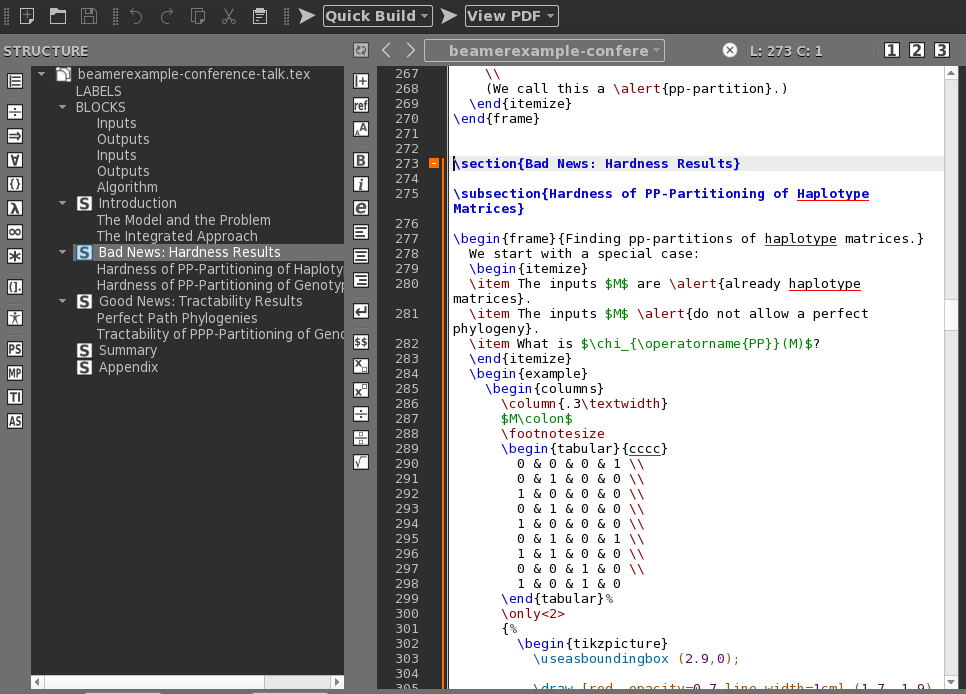
\includegraphics[width=0.70\linewidth]{../Norme_di_progetto/img/texMaker.png}
	\caption{\TeX{}maker - per la stesura dei documenti}
\end{figure}

\paragraph{GanttProject}\mbox{} \\ \mbox{} \\
GanttProject è un programma gratuito dedicato alla produzione dei diagrammi di Gantt\glo. Permette di creare task e milestone\glo, organizzare le task in lavoro strutturato a interruzioni, disegnare
i vincoli di dipendenza tra di esse e molte altre utilità, generando automaticamente il relativo diagramma. \\
\centerline{\url{https://www.ganttproject.biz/}}
\begin{figure}[H]
	\centering
	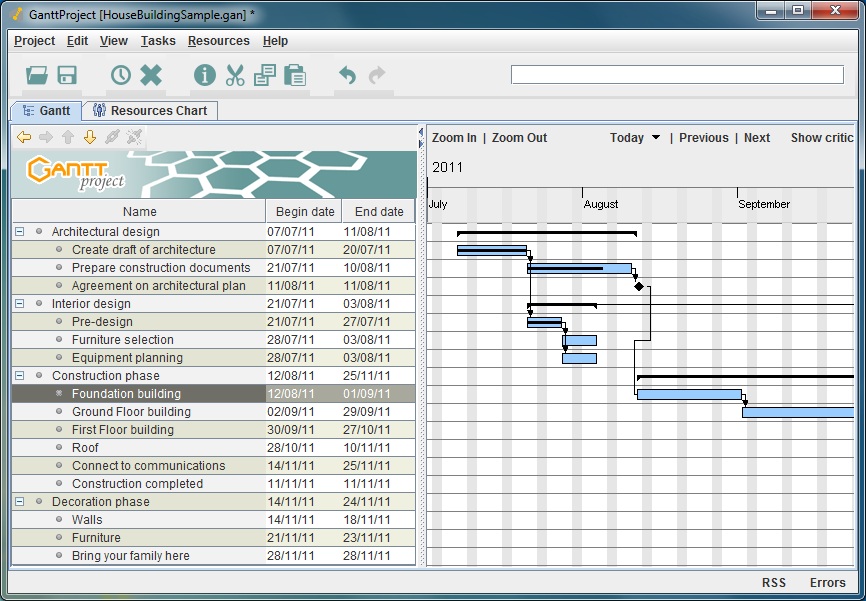
\includegraphics[width=0.70\linewidth]{../Norme_di_progetto/img/gantt.png}\\
			\caption{GanttProject - per la relizzazione di diagrammi di Gantt}
\end{figure}

\paragraph{Draw.io}\mbox{} \\ \mbox{} \\
Draw.io viene utilizzato per la produzione degli UML.\\
\centerline{\url{https://www.draw.io/}} 

\subsection{Gestione della configurazione}
\subsubsection{Scopo}
L'obiettivo della configurazione è di creare ordine tra i documenti e il software. Tutto ciò che è configurato ha uno stato identificativo, è modificato secondo regole ben definite ed è posto sotto versionamento\glo.

\subsubsection{Aspettative}
Questa sezione ha lo scopo supportare i processi di documentazione, di sviluppo e manutenzione del software rendendoli definiti e ripetibili.
\subsubsection{Attività}

\paragraph{Versionamento}\mbox{} \\ \mbox{} \\
Ogni versione di qualsiasi documento deve corrispondere ad una riga della tabella delle modifiche. Il numero di versione è composto da tre cifre: \\ \\
\centerline{X.Y.Z} \\
\begin{itemize}
\item \textbf{X}: rappresenta una versione stabile del documento, resa tale dopo l'approvazione del \textit{Responsabile} di progetto: \begin{itemize}
\item inizia da 0; 
\item viene incrementata di un'unità alla volta.
\end{itemize}
\item \textbf{Y}: indica l'ultima versione del documento che ha passato la fase di verifica: \begin{itemize}
\item inizia da 0;
\item viene incrementato dal verificatore ad ogni verifica;
\item quando viene incrementato X, viene riportato a 0.
\end{itemize} 
\item \textbf{Z}: indica l'ultima modifica apportata al documento dal redattore: \begin{itemize}
\item inizia da 0;
\item viene incrementato dal redattore del documento ad ogni modifica;
\item quando viene incrementato Y, viene riportato a 0.
\end{itemize}
\end{itemize}
Apprese le correzioni effettuate dal docente, il \textit{TeamAFK} ha deciso di modificare il significato che questi parametri assumevano, consentendo di ottenere uno scatto di versione solo successivamente ad un'operazione di verifica. Il significato che i nuovi parametri assumono sono:
\begin{itemize}
    \item \textbf{X}: un suo aumento determina che il documento sia stato modificato, verificato e approvato, quindi ritenuto pronto al rilascio;
    \item \textbf{Y}: un suo aumento determina la conclusione di un'attività di modifica e di verifica di un processo ritenuto di entità maggiore, come può essere l'inserimento di una nuova sezione o la sua modifica;
    \item \textbf{Z}: un suo aumento determina la conclusione di un'attività di modifica e di verifica di un processo ritenuto di entità minore, come può essere una correzione o un'aggiunta.
\end{itemize}
L'aumento del parametro X determina l'azzeramento dei parametri Y e Z.


\paragraph{GitHub}\mbox{} \\ \mbox{} \\
Per le parti del progetto da versionare si è scelto di usare GitHub\glo, un servizio del sistema di versionamento distribuito Git per contenere la repository remota. \\
I membri del team possono interagire con il VCS\glo sia da linea di comando, sia attraverso software che ne migliorano l'usabilità, come GitKraken e GitHub Desktop. La versione ufficiale del progetto è ospitata in una repository remota su GitHub, all'indirizzo \\
\centerline{\url{https://github.com/teamafkSWE}}

\subparagraph{Struttura del repository} \mbox{} \\ \mbox{} \\
All'interno della repository principale sopra descritta troviamo due differenti repository: \begin{itemize}
\item \textbf{PredireInGrafana-docs}: contiene tutti i documenti ufficiali del progetto, suddivisi in specifiche cartelle: \\
\centerline{\url{https://github.com/teamafkSWE/PredireInGrafana-docs}}  \begin{itemize}
\item \textbf{Cartella principale - Presentazioni}: raccoglie le presentazioni relative ad ogni consegna;
\item \textbf{Cartella principale - RR}: raccoglie i file sorgenti per la compilazione dei documenti, suddivisi tra esterni ed interni, realizzati per la \textit{Revisione dei Requisiti};
\item \textbf{Cartella principale - RP}: raccoglie i file sorgenti per la compilazione dei documenti, suddivisi tra esterni ed interni, realizzati per la \textit{Revisione di Progettazione}. In futuro saranno aggiunte cartelle distinte nominate \textbf{RQ} e \textbf{RA}, contenenti i file delle rispettive consegne.
\begin{itemize}
\item[$\bullet$] \textbf{Tipologia\_di\_documento}: ogni documento avrà la rispettiva cartella (e.i. Norme\_di\_progetto), contenente tutti i file (sezioni ed immagini) necessari per la sua compilazione;
\item[$\bullet$] \textbf{copertina.tex}: file che permetterà una facile e rapida modifica dell'impostazione testuale del frontespizio.
\end{itemize}
\item \textbf{Template}: contiene tutti i file che definiscono il template \LaTeX{} per la creazione di nuovi documenti.
\end{itemize} 
\item \textbf{PredireInGrafana-SW}: conterrà tutti i file di codifica dei plug-in da sviluppare. \\ \centerline{\url{https://github.com/teamafkSWE/PredireInGrafana-SW}}
\end{itemize}
Entrambe le repository, avranno una propria struttura identica a livello: \begin{itemize}
\item \textbf{Locale}: ogni membro del gruppo lavora sui file clonati dal repository remoto nel proprio PC;
\item \textbf{Remoto}: presente su GitHub, contiene il lavoro svolto da ogni componente e che viene condiviso con il team.
\end{itemize}

\subparagraph{Tipi di file} \mbox{} \\ \mbox{} \\
I file utilizzati per la documentazione del progetto sono: \begin{itemize}
\item file con estensione .tex di \LaTeX{};
\item file con estensione .pdf (da consegnare);
\item file di stile, .sty,  e immagini di supporto.
\end{itemize}
Il file ".gitignore" è presente al livello più esterno della repository ed elenca tutti i file esclusi dal versionamento.

\subparagraph{Utilizzo di Git} \mbox{} \\ \mbox{} \\
Il repository di Git è composto da vari branch\glo, per favorire la collaborazione tra i vari membri e il parallelismo delle attività. Si consiglia quindi di seguire questa procedura:
\begin{enumerate}
\item scegliere il proprio branch di lavoro;
\item eseguire il pull\glo dal repository remoto, che effettua quindi l'aggiornamento del proprio repository locale;
\item svolgere il compito assegnato;
\item eseguire il comando di aggiunta (add) dei file nuovi o modificati da condividere all'area di staging\glo;
\item eseguire il comando di commit\glo dei file aggiunti, corredato da un messaggio che identifica il lavoro svolto;
\item eseguire il push\glo del commit sul repository remoto.
\end{enumerate}

\paragraph{Gestione delle modifiche}\mbox{} \\ \mbox{} \\
Tutti i membri del team possono modificare i file in ogni branch, ad eccezione del branch master, per il quale occorre richiedere una pull e ottenere l'approvazione di un altro membro. \\
Per effettuare modifiche maggiori sui contenuti o sulla struttura dei file è previsto: \begin{itemize}
\item contattare il \textit{Responsabile} del file da modificare;
\item suggerire la modifica da effettuare;
\item se il responsabile valuta positivamente la modifica, allora la applica.
\end{itemize}
Per modifiche minori, come correzioni grammaticali o miglioramenti sintattici, si consiglia di modificare indipendentemente. In entrambi i casi è opportuno commentare i propri commit con chiarezza per risalire facilmente alle modifiche effettuate.

\paragraph{Metriche di qualità}\mbox{} \\ \mbox{} \\
Per questo processo non sono state definite metriche di qualità.

\paragraph{Strumenti di supporto}
\subparagraph{GitHub}\mbox{} \\ \mbox{} \\
In aggiunta ai servizi già elencati, al fine di migliorare efficacia ed efficienza, vengono utilizzate le funzionalità di "Issue Tracking System", "Milestone" e "Project Board" integrate in GitHub. Ognuna di queste funzionalità viene usata solo da chi autorizzato, ad esempio rilasci di versioni, creazione e chiusura di milestone sono concesse solo al \textit{Responsabile di Progetto}.\\
Vengono inoltre utilizzate le "Labels" offerte dall’Issue Tracking System di Github per definire le tipologie di problemi e le loro priorità.\\
Per il repository contenente il codice sorgente del software sono utilizzate le GitHub Actions al fine di implementare la pratica della continuous integration che, a sua volta, utilizza strumenti quali Coveralls per eseguire le verifiche automatiche sul codice sorgente.

\subparagraph{Coveralls}\mbox{} \\ \mbox{} \\
Servizio web utilizzato per tenere traccia della copertura del codice.\\
	\centerline{\url{https://coveralls.io/}}

\subsection{Gestione della qualità}
\subsubsection{Scopo}
Lo scopo è garantire che il prodotto e i servizi offerti rispettino gli obiettivi di qualità e che i bisogni del proponente siano soddisfatti. 

\subsubsection{Aspettative}
Le aspettative di questo processo sono riassunte nei seguenti punti che rappresentano gli obiettivi che vogliono essere raggiunti. Si vuole ottenere: \begin{itemize}
\item qualità per tutta la durata del ciclo di vita del software;
\item garanzia di raggiungimento degli obiettivi di qualità prestabiliti;
\item soddisfazione del cliente in merito al prodotto sviluppato;
\item oggettività nella ricerca della qualità in modo da ottenerla in tutti i processi e in tutti i prodotti;
\item qualità misurabile attraverso delle metriche.
\end{itemize}

\subsubsection{Descrizione}
La gestione della qualità viene approfondita nel \textit{Piano di Qualifica}, dove sono descritte le modalità utilizzate per garantire la qualità nello sviluppo del progetto. In particolare: \begin{itemize}
\item sono presentati gli standard utilizzati;
\item sono individuati i processi\glo di interesse;
\item sono individuati gli attributi del software più importanti per il progetto.
\end{itemize}
Per ogni processo vengono descritti: \begin{itemize}
\item gli obiettivi da perseguire;
\item le strategie da applicare;
\item le metriche da utilizzare.
\end{itemize}
L'obiettivo è ottenere software e documentazione di qualità soddisfacente.

\subsubsection{Attività}
\paragraph{Classificazione delle metriche} \mbox{} \\  \mbox{} \\ 
Le metriche sono distinte in tre categorie: processi, documentazione e codifica. Per ciascuna di esse si indica il motivo per cui è stata scelta e la procedura di calcolo.  \\
Le metriche rispetteranno la seguente notazione: \\
\centerline{\textbf{M[categoria][numero]}}
dove: \begin{itemize}
\item Categoria: indica la categoria della metrica, più precisamente:
\begin{itemize}
\item \textbf{P} per indicare le metriche dei processi;
\item \textbf{D} per indicare le metriche dei documenti;
\item \textbf{S} per indicare le metriche della codifica del software e dei relativi test.
\end{itemize}
\item numero: identifica in maniera univoca la metrica in ogni categoria, assume un valore intero a due cifre incrementale, a partire da 01.
\end{itemize}
Se nelle formule di calcolo delle metriche è presente il simbolo "\#", va inteso come la parola "numero". Un esempio può essere il seguente:
\[ \#parole\_doc = numero\ di\ parole\ presenti\ nel\ documento \]

\subsubsection{Metriche di qualità}
\paragraph*{PROC - Percentuale di metriche soddisfatte}\mbox{} \\ \mbox{} \\ 
Indica la percentuale di metriche soddisfatte rispetto alla totalità di metriche da utilizzare all’interno del progetto. Si calcolo con la seguente formula:
\[ PROC = \frac{metriche\_soddisfatte}{metriche\_totali} \]

\subsubsection{Strumenti di supporto}
Gli strumenti di supporto utilizzati per garantire la qualità sono le metriche di qualità.


\subsection{Verifica}
\subsubsection{Scopo}
Il processo di verifica ha come scopo la realizzazione di prodotti corretti, coesi e completi. Sono soggetti a verifica i documenti e il software.
Il processo di verifica deve rispettare i seguenti punti: \begin{itemize}
\item la verifica deve essere effettuata seguendo procedure ben definite;
\item per verificare vi sono criteri chiari e affidabili;
\item ogni fase del prodotto viene verificata;
\item dopo la verifica il prodotto è in uno stato stabile;
\item il prodotto può essere validato.
\end{itemize}

\subsubsection{Aspettative}
La verifica viene effettuata per raggiungere i seguenti obiettivi: \begin{itemize}
\item cercare consistenza, completezza e correttezza nelle singole attività;
\item ottenere supporto per una successiva validazione del prodotto;
\item avere a disposizione dei criteri e procedure, comprensibili e affidabili, da seguire.
\end{itemize}

\subsubsection{Descrizione}
Il processo di verifica assicura che tutte le attività svolte della fase in esame, attraverso analisi e test successivamente definiti, siano conformi alle aspettative; prende in input ciò che è già stato prodotto e lo restituisce in uno stato stabile. \\
Per ottenere tale risultato ci si affida a processi di analisi e test.

\subsubsection{Attività}
Le attività che si effettuano durante la verifica sono due tipi di analisi: l’analisi statica e l’analisi dinamica.

\paragraph{Analisi statica} \mbox{} \\ \mbox{} \\
L'analisi statica effettua controlli su documenti e codice. Questo tipo di analisi serve per rilevare varie tipologie di anomalie. \\
Questa attività viene effettuata con l'ausilio di due metodi manuali di lettura (attuati da persone) differenti: \begin{itemize}
\item \textbf{Walkthrough}: i vari componenti del team effettuano una lettura scrupolosa di documenti e/o codice alla ricerca di errori, senza sapere inizialmente se ce ne siano;
\item \textbf{Inspection}: i verificatori usano liste di controllo (checklist) per fare ispezione cercando errori specifici in parti specifiche. Questa tecnica permette quindi di aumentare l'efficienza dello sviluppo, diminuendo i tempi dell'analisi statica.
\end{itemize}
A seguire sono descritte le liste di controllo utilizzabili per le ispezioni:
\begin{table}[H]
\caption{Errori frequenti nei documenti}
\begin{center}
\begin{tabular}{C{4.5cm} C{11cm}}
\rowcolor{redafk}
\textcolor{white}{\textbf{Oggetto}} & \centerline{\textcolor{white}{\textbf{Controllo}}} \\
Formato data & Deve seguire il formato gregoriano YYYY-MM-DD. \\
Sintassi & La frase è troppo complessa e deve essere semplificata. \\
Punteggiatura degli elenchi & Ogni voce termina in ";" eccetto l'ultima che termina in ".".\\
Errori di battitura & Tipici errori di battitura dovuti alla vicinanza delle
lettere sulla tastiera, ad esempio la lettera "a" al posto della "s", "i" al posto di "o", "m" al posto di "n". \\
Uso degli accenti & Utilizzare le lettere accentate presenti nella tastiera o utilizzare il codice ALT. \\
Inconsistenze nell’uso delle iniziali maiuscole nei titoli delle parti di documento & Ogni titolo deve avere la prima lettera della prima parola maiuscola e il resto minuscolo, tranne quando ci si riferisci ad attività o documenti specifici. \\
Gerarchia delle sezioni & Non viene scritta la gerarchia delle sezioni dei documenti in maniera adeguata, ovvero: section, subsection, subsubsection, paragraph, subparagraph, subsubparagraph. \\
\end{tabular}
\end{center}
\end{table}

\paragraph{Analisi dinamica} \mbox{} \\ \mbox{} \\
L'analisi dinamica è una tecnica di analisi del prodotto software che richiede la sua esecuzione. Produce una misura della qualità del prodotto, mediante l'esecuzione di test specifici che verificano se il prodotto funziona e se ci sono anomalie.

\subparagraph{Test} \mbox{} \\ \mbox{} \\
I test sono l'attività fondamentale dell'analisi dinamica: il loro scopo è verificare che il codice
scritto funzioni correttamente. I test devono:
\begin{itemize}
\item essere ripetibili;
\item specificare l'ambiente di esecuzione;
\item identificare input e output richiesti;
\item avvertire di possibili effetti indesiderati;
\item fornire informazioni sui risultati dell'esecuzione.
\end{itemize}
Ci sono vari tipi di test, ognuno dei quali ha un diverso oggetto di verifica e scopo.

\paragraph*{Test funzionali} \mbox{} \\ \mbox{} \\
Test condotti per valutare la conformità di un componente o sistema con requisiti\glo funzionali. Ne fanno parte: \begin{itemize}
\item \textbf{Test di unità}: si eseguono su unità di software, e si concentrano sul loro funzionamento individuale;
\item \textbf{Test di integrazione}: verificano se sono rispettati i contratti di interfaccia tra più moduli o sub-system (interni o esterni);
\item \textbf{Test di accettazione}: gli UAT (User Acceptance Testing) si occupano di verificare il prodotto e, in particolare, il soddisfacimento del cliente. Il superamento di questi test garantisce che il software sia pronto per essere rilasciato.
\end{itemize}

\paragraph*{Test di regressione} \mbox{} \\ \mbox{} \\
Il test di regressione va eseguito ogni volta che viene modificata un'implementazione in un programma. È possibile eseguire nuovamente i test esistenti sul codice modificato, integrando solo le parti che abbiano precedentemente superato il test di unità, per stabilire se le modifiche apportate hanno alterato elementi precedentemente funzionanti.\\ Se necessario è anche possibile scrivere nuovi test.

\paragraph*{Test di sistema} \mbox{} \\ \mbox{} \\
Verificano il comportamento dell'intero sistema.\\
Lo scopo principale di questi test è la verifica del sistema rispetto alle specifiche tecniche definite nel'\textit{Analisi dei Requisiti}.

\subparagraph*{Codifica dei test} \mbox{} \\ \mbox{} \\
La codifica dei test è la seguente: \\
\centerline{\textbf{TX[Tipo\_Requisito][Importanza][CodiceUC]}}
dove: \begin{itemize}
\item \textbf{X}: indica il tipo di test. Può assumere i seguenti valori: \begin{itemize}
\item \textbf{U}: indica un test di unità;
\item \textbf{I}: indica un test di integrazione;
\item \textbf{A}: indica un test di accettazione;
\item \textbf{R}: indica un test di regressione;
\item \textbf{S}: indica un test di sistema.
\end{itemize} 
\item \textbf{Tipo\_Requisito}: indica il tipo del requisito. Esso può essere: \begin{itemize}
\item \textbf{O}: obbligatorio;
\item \textbf{D}: desiderabile;
\item \textbf{F}: facoltativo.
\end{itemize}
\item \textbf{Importanza}: indica l'importanza del requisito. Viene indicata con: \begin{itemize}
\item \textbf{F}: per indicare un requisito funzionale;
\item \textbf{V}: per indicare un requisito di vincolo;
\item \textbf{Q}: per indicare un requisito di qualità;
\item \textbf{P}: per indicare un requisito prestazionale.
\end{itemize}
\item \textbf{CodiceUC}: rappresenta il codice identificativo crescente del componente da verificare.
\end{itemize}

\subsubsection{Metriche di qualità} \label{sez:meVe}
Le metriche descritte in questa sezione sono metriche software utilizzate per verificare la qualità e la completezza dei test effettuati. Più in dettaglio:
\begin{longtable}{ C{4.5cm} c L{9.5cm} }
	\rowcolor{white}\caption{Metriche per la qualità e completezza dei test}\\
		\rowcolor{redafk}
		\textcolor{white}{\textbf{Nome}} & \textcolor{white}{\textbf{Codice}} & \centerline{\textcolor{white}{\textbf{Descrizione}}} \\
		\endfirsthead
		\rowcolor{white}\caption[]{(continua)} \\
		\rowcolor{redafk}
		\textcolor{white}{\textbf{Nome}} & \textcolor{white}{\textbf{Codice}} & \centerline{\textcolor{white}{\textbf{Descrizione}}} \\
		\endhead
		Code Coverage (CC) & MS07 & Percentuale delle linee di codice coperte dai test. Avere codice coperto da test riduce la possibilità di introdurre errori nel prodotto. 
		\[ CC[\%] = \frac{\#righe\_codice\_testate}{\#tot\_righe\_codice}\] \\
		Passed Test Cases Percentage (PTCP) & MS08 & Percentuale di test superati sul totale dei test eseguiti. Un'alta percentuale di superamento indica la tendenza del codice ad essere già corretto prima dei test. Si calcola con la seguente
formula:
		\[ PTCP[\%] = \frac{\#test\_superati}{\#test\_eseguiti}\cdot 100 \] \\
		Failed Test Cases Percentage (FTCP) & MS09 & Percentuale di test falliti sul totale dei test eseguiti. Un'alta percentuale di fallimento indica la tendenza
alla scorrettezza del codice. Si calcola con la seguente formula:
\[ FTCP[\%] = \frac{\#test\_falliti}{\#test\_eseguiti}\cdot 100 \] \\
\end{longtable}

\subsubsection{Strumenti di supporto}

\paragraph{Correzione ortografica} \mbox{} \\ \mbox{} \\
Il controllo ortografico viene eseguito principalmente basandosi sugli strumenti integrati in \TeX{}maker, il quale fornisce un dizionario italiano e sottolinea in rosso le parole che non vi appartengono. 

\paragraph{Coveralls} \mbox{} \\ \mbox{} \\
Coveralls è uno strumento che permette di quantificare la percentuale di codice testato.

\subsection{Validazione}
\subsubsection{Scopo}
Lo scopo del processo di validazione è  accertare che il prodotto finale corrisponda alle attese, soddisfando tutti i requisiti concordati e i bisogni del committente.

\subsubsection{Aspettative}
Le aspettative del \textit{TeamAFK} sono di normare adeguatamente il processo di validazione al fine di rilasciare un prodotto privo di errori gravi e capace di rispondere alle richieste del proponente.

\subsubsection{Descrizione}
Le attese sono quelle del committente e corrispondono all’\textit{analisi\_dei\_requisiti\_v3.0.0}. Per eseguire una validazione si deve avere un prodotto ad un sufficiente livello di avanzamento, quindi il numero di validazioni svolte è minore rispetto al numero delle verifiche. Durante questo processo vengono svolti i test di accettazione tramite i quali il proponente valida il prodotto software.

\subsubsection{Attività}
\paragraph{Test di accettazione}\mbox{} \\ \mbox{} \\
Gli UAT si occupano di verificare il prodotto e, in particolare, il soddisfacimento del cliente. Il superamento di questi test garantisce che il software sia pronto per essere rilasciato.

\subsubsection{Metriche di qualità}
Per questo processo non sono state definite particolari metriche di qualità.

\subsubsection{Strumenti di supporto}
Per questo processo non vengono utilizzati degli strumenti di supporto.

\subsection{Gestione dei cambiamenti}
\subsubsection{Scopo}
Lo scopo di questo processo è fornire un metodo tempestivo, disciplinato e documentato per assicurare che tutti i cambiamenti, compresi i problemi, riscontrati nel corso del progetto, siano identificati, analizzati e risolti.

\subsubsection{Aspettative}
Questo approccio porta i seguenti vantaggi, fondamentali per rispettare il \textit{Piano di Progetto}: 
\begin{itemize}
\item rispetto degli obiettivi prefissati;
\item rispetto dei tempi previsti;
\item rispetto del budget preventivato.
\end{itemize}

\subsubsection{Descrizione}
Il Change Management è un approccio strutturato al cambiamento negli individui, nei gruppi e nelle organizzazioni che rende possibile la transizione da un assetto corrente a un futuro assetto desiderato.
Un programma strutturato di sviluppo e crescita delle risorse umane è un elemento fondamentale di accompagnamento al cambiamento.\\ Pertanto, il \textit{TeamAFK} ha scelto di seguire l'approccio \textbf{agile} per la gestione del progetto, in cui i requisiti e le soluzioni maturano in corso d’opera attraverso la collaborazione fra stakeholders. Si tratta quindi di produrre il più rapidamente possibile i prototipi e poi rifinirli attraverso cicli successivi di miglioramento.

\subsubsection{Attività}
\paragraph{Adattamento ed implementazione del processo}\mbox{} \\ \mbox{} \\
Per avvalorare quanto detto prima ed implementare tale processo al progetto in corso, il \textit{TeamAFK} ha deciso di adottare il modello 4P: \begin{itemize}
\item \textbf{People}: il Change Management efficace mette l'utente al centro. Il \textit{Responsabile del Progetto} gestisce le comunicazioni interne tra i membri del gruppo e quelle esterne con il proponente e/o committente;
\item \textbf{Process}: i processi vengono rivisti in chiave moderna ed efficace; devono essere circolari e chiusi, assicurando che: \begin{itemize}
\item tutti i cambiamenti siano prontamente segnalati e gestiti tramite il processo di risoluzione dei cambiamenti;
\item i cambiamenti vengano presi in carico e gestiti;
\item vengano inviate delle notifiche per informare gli interessati della presenza dell’eventuale problema;
\item le cause del problema vengano identificate, analizzate e, dove possibile, eliminate;
\item la risoluzione e le decisioni prese siano archiviate e storicizzate;
\item lo stato del cambiamento sia tracciato, aggiornato e comporti delle notifiche al cambio di stato;
\item venga mantenuto un registro di tutti i problemi riscontrati.
\end{itemize}
\item \textbf{Platform}: il \textit{TeamAFK} utilizza tecnologie avanzate a supporto dello sviluppo del progetto (ESLint, Coveralls, TravisCI);
\item \textbf{Place}: si intendono i luoghi di lavoro dove viene svolto il progetto. Il \textit{TeamAFK} si vede obbligato in questo senso ad attuare lo Smart Working, a causa delle limitazioni dovute da Covid19.
\end{itemize}
La modalità di gestione e di risoluzione individuate per i cambiamenti e per i problemi sono analizzate e valutate al fine di verificare che siano stati effettivamente risolti e che le modifiche siano state correttamente implementate nei prodotti software e nelle attività. Inoltre l’analisi deve permettere di individuare dei pattern di risoluzione ed aiutare a determinare quando vengono introdotti ulteriori problemi.
\paragraph{Risoluzione dei problemi}\mbox{} \\ \mbox{} \\
Quando dei cambiamenti, problemi compresi, sono rilevati in un prodotto software o in un’attività, deve essere realizzato un report che li descriva. Questo report deve essere usato come componente del punto precedente: dall’individuazione dei cambiamenti al processo di analisi e risoluzione, fino all’individuazione della causa ed alla sua analisi per individuarne la natura. Per svolgere quanto descritto, ci si appoggia all’Issue Tracking System di GitHub. Esso consente di aggiungere delle issues che corrispondono ai cambiamenti o ai problemi che si devono svolgere e di assegnarle ad incaricati e responsabili.

\subsubsection{Metriche di qualità}
Per questo processo non sono state definite delle metriche di qualità specifiche.

\subsubsection{Strumenti di supporto}
Per questo processo non vengono utilizzati degli strumenti di supporto.

\pagebreak
	
\section{Processi Organizzativi}

\subsection{Gestione di Progetto}

\subsubsection{Ruoli di progetto}
Ciascun membro del gruppo, a rotazione, deve ricoprire il ruolo che gli viene assegnato e che corrisponde all'omonima figura aziendale. Nel \textit{Piano di Progetto}\glo vengono organizzate e pianificate le attività assegnate agli specifici ruoli. I ruoli che ogni componente del gruppo è tenuto a rappresentare sono descritti di seguito.

\paragraph{Responsabile di progetto}\mbox{} \\ \mbox{} \\
Il \textit{Responsabile di progetto} (o semplicemente \textit{Responsabile}) è una figura chiave in quanto ricadono su di lui le responsabilità di pianificazione, gestione, controllo e coordinamento delle risorse e attività del gruppo. Il \textit{Responsabile} si occupa anche di interfacciare il gruppo con le persone esterne facendo da intermediario: sono quindi di sua competenza le comunicazioni con committente e proponente.
Questa figura è incaricata anche di analizzare e gestire le criticità, che si incontrano durante il progetto, e di approvare i documenti.

\paragraph{Amministratore di progetto}\mbox{} \\ \mbox{} \\
L'\textit{Amministratore} ha il compito di supporto e controllo dell'ambiente di lavoro.
Egli deve quindi:
\begin{itemize}
	\item dirigere le infrastrutture di supporto;
	\item risolvere problemi legati alla gestione dei processi;
	\item gestire la documentazione;
	\item controllare versioni e configurazioni.
\end{itemize}

\paragraph{Analista}\mbox{} \\ \mbox{} \\
L'\textit{Analista} si occupa di analisi dei problemi e del dominio applicativo. Questa figura ha anche il compito di redigere i documenti, in questo caso può essere definito come \textit{Redattore}.
Le sue responsabilità sono:
\begin{itemize}
	\item studio del dominio del problema;
	\item definizione della complessità e dei requisiti dello stesso;
	\item redazione del documenti:\textit{ Analisi dei Requisiti} e \textit{Studio di Fattibilità}.
\end{itemize}

\paragraph{Progettista}\mbox{} \\ \mbox{} \\
Il \textit{Progettista} gestisce gli aspetti tecnologici e tecnici del progetto.
Il \textit{Progettista} deve:
\begin{itemize}
	\item effettuare scelte efficienti ed ottimizzate su aspetti tecnici del progetto;
	\item sviluppare un'architettura che sfrutti tecnologie note ed ottimizzate, su cui basare un prodotto stabile e manutenibile.
\end{itemize}

\paragraph{Programmatore}\mbox{} \\ \mbox{} \\
Il \textit{Programmatore} è responsabile della codifica del progetto e delle componenti di supporto che serviranno per effettuare le prove di verifica e validazione sul prodotto.
Il \textit{Programmatore} si occupa di:
\begin{itemize}
	\item implementare le decisioni del progettista;
	\item creare o gestire componenti di supporto per la verifica e validazione del codice.
\end{itemize}

\paragraph{Verificatore}\mbox{} \\ \mbox{} \\
Il \textit{Verificatore} si occupa di controllare il prodotto del lavoro svolto dagli altri membri del team, sia esso codice o documentazione. Per le correzioni si affida agli standard definiti nelle \textit{Norme di Progetto}, nonché alla propria esperienza e capacità di giudizio.
Il \textit{Verificatore} deve:
\begin{itemize}
	\item ispezionare i prodotti in fase di revisione, avvalendosi delle tecniche e degli strumenti definiti nelle \textit{Norme di Progetto};
	\item evidenziare difetti ed errori del prodotto in esame;
	\item segnalare eventuali errori trovati all'autore dell'oggetto preso in esame o alla persona che ha responsabilità su di esso.
\end{itemize}

\subsubsection{Gestione dei rischi}
È compito del \textit{Responsabile} rilevare i rischi e renderli noti, tramite un continuo monitoraggio e una continua identificazione di quest'ultimi. \\
Qualora dovesse essere \textbf{identificato} un nuovo rischio è necessario procedere con i seguenti passaggi:
\begin{enumerate}
	\item \textbf{Classificare} il rischio seguendo la codifica;
	\item \textbf{Descrivere} una strategia da applicare per gestire il rischio;
	\item \textbf{Riportare} il rischio nel \textit{Piano di Progetto}.
\end{enumerate}

\paragraph{Codifica}\mbox{} \\ \mbox{} \\
La codifica dei rischi è utilizzata per la classificazione. Il codice di un rischio si presenta nella forma: \\
\centerline{\textbf{Ri[Categoria][Grado][Numero]}}
dove:
\begin{itemize}
	\item \textbf{Categoria}: indica la categoria del rischio, essa può assumere i valori:
	\begin{itemize}
		\item \textbf{O} per i rischi organizzativi;
		\item \textbf{T} per i rischi tecnologici;
		\item \textbf{P} per i rischi interpersonali.
	\end{itemize}
	\item \textbf{Grado}: indica il grado di rischio, è la somma tra la probabilità e la gravità. Queste ultime possono assumere i seguenti valori:
	\begin{itemize}
		\item \textbf{0}: bassa;
		\item \textbf{1}: media;
		\item \textbf{2}: alta.
	\end{itemize}
	(In questo caso un rischio con una probabilità bassa ma una gravità alta avrà lo stesso grado di un rischio con una probabilità alta e una gravità bassa, ovvero 2)
	\item \textbf{Numero}: insieme a categoria e grado identifica in maniera univoca il rischio, può assumere un valore intero progressivo ad una cifra (0-9).
\end{itemize}

\subsection{Processi di Coordinamento}
Di seguito vengono descritte le norme che regolano le comunicazioni e gli incontri del gruppo, che siano tra i membri o con committenti e proponenti.
\subsubsection{Gestione Comunicazioni}
\paragraph{Comunicazioni Interne}\mbox{} \\ \mbox{} \\
Le comunicazioni interne ai membri del gruppo vengono gestite  tramite 2 applicazioni:
\begin{itemize}
	\item Telegram\glo;
	\item Discord\glo.
\end{itemize}
È stato disposto un gruppo Telegram sul quale si discute di tematiche generali o collettive, garantendo risposte rapide e ordinate in caso di decisioni per votazione, grazie ad apposite funzioni dette bot di Telegram\glo. \\
Discord viene usato principalmente per le riunioni tra i membri del gruppo, ma l'applicazione mette anche a disposizione dei canali testuali. Tali canali sono stati suddivisi per tema e vengono usati per le comunicazioni specifiche per agevolare la stesura dei documenti. Vengono suddivisi in:
\begin{itemize}
	\item \textbf{General}: per discussioni riguardanti rotazioni dei ruoli e decisione degli argomenti da discutere nelle riunioni;
	\item \textbf{Links}: per tenere traccia di tutti i link utili al progetto;
	\item \textbf{Analisi-requisiti}: per discutere gli Use Case\glo e i requisiti necessari alla stesura dell'\textit{Analisi dei Requisiti};
	\item \textbf{Norme}: per discutere riguardo le regole del \textit{Way of Working} del gruppo, le norme da seguire e, di conseguenza, la stesura del documento \textit{Norme di Progetto}\glo;
	\item \textbf{Piano-progetto}: per confrontarsi riguardo il monte ore dei vari ruoli e per facilitare la stesura del documento \textit{Piano di Progetto};
	\item \textbf{Piano-qualifica}: per discutere di strategie da attuare per garantire qualità attraverso verifica\glo e validazione\glo.
\end{itemize}
\paragraph{Comunicazioni Esterne}\mbox{} \\ \mbox{} \\
Le comunicazioni con soggetti esterni al gruppo sono di competenza del responsabile. Gli strumenti predefiniti sono la posta elettronica, dove viene utilizzato l'indirizzo \href{mailto:gruppoafk15@gmail.com}{gruppoafk15@gmail.com}.
Per comunicare con \textit{Zucchetti SPA} viene usato il servizio Skype\glo per le chiamate. Il responsabile ha il compito di tenere informati gli altri componenti del gruppo in caso di assenza.

\subsubsection{Gestione Riunioni}
Le riunioni possono essere interne o esterne. All'inizio di ogni riunione il \textit{Responsabile} nomina, tra i componenti del gruppo, un \textit{Segretario} che si occuperà di far rispettare l'ordine del giorno. Inoltre ha l'onere della stesura del \textit{Verbale di Riunione}\glo.

\paragraph{Riunioni interne} \mbox{} \\ \mbox{} \\
E' compito del \textit{Responsabile} organizzare riunioni interne al gruppo. Ciò prevede, più nello specifico, la stesura dell'ordine del giorno e
stabilire data, orario e luogo di incontro, mediando se necessario con i membri per permettere la presenza di tutti. Le riunioni sono tenute principalmente usando Discord, così da essere il più facilmente raggiungibili.
Il \textit{Responsabile} deve inoltre assicurarsi, attraverso la comunicazione
mediante i mezzi propri del gruppo, che ogni componente sia pienamente a conoscenza della riunione in tutti i suoi dettagli. \\
D'altro canto ogni membro del gruppo deve presentarsi puntuale agli appuntamenti,
e comunicare in anticipo eventuali ritardi o assenze adeguatamente giustificate.

\paragraph{Riunioni esterne} \mbox{} \\ \mbox{} \\
E' nuovamente compito del \textit{Responsabile} organizzare riunioni esterne.
Nello specifico egli deve preoccuparsi di contattare l'azienda proponente per fissare gli
incontri e qualora sia necessario, tenendo conto anche delle preferenze di date e orario
espresse dagli altri membri del gruppo. La partecipazione a tali riunioni deve essere,
a meno di casi eccezionali, unanime.
Ogni membro del gruppo può, inoltre, esprimere al Responsabile una richiesta, adeguatamente motivata, di fissare una riunione esterna. A questo punto sarà compito
dello stesso Responsabile giudicare come valida o meno la richiesta presentatagli ed
agire di conseguenza.

\paragraph{Verbale di riunione} \mbox{} \\ \mbox{} \\
Ad ogni riunione, interna o esterna, è compito del \textit{Segretario} designato redigere il \textit{Verbale di riunione} corrispondente, che deve essere poi approvato dal \textit{Responsabile}. La struttura del \textit{Verbale} è definita in \hyperref[par:verbali]{§ 3.5.5}.


\subsection{Strumenti}
Il gruppo, nel corso del progetto, ha utilizzato o utilizzerà i seguenti strumenti:
\begin{itemize}
	\item \textbf{Telegram}: strumento di messaggistica usato per comunicazioni veloci tra i membri; 
	\item \textbf{Discord}: per comunicazioni specifiche o per riunioni interne;
	\item \textbf{Git}: sistema di controllo di versionamento;
	\item \textbf{Gitflow}: sistema per agevolare varie operazioni su Git;
	\item \textbf{GitHub}: per il versionamento e il salvataggio in remoto di tutti i file riguardanti il progetto;
	\item \textbf{GanttProject}: software OpenSource\glo usato per la realizzazione dei diagrammi di Gantt;
	\item \textbf{Google Doc}: editor di testo cloud, usato per tenere degli appunti modificabili da tutti;
	\item \textbf{Google Drive}: utilizzato per il salvataggio in remoto dei file non sottoposti a versionamento, in modo da essere reperibili a tutti i membri;
	\item \textbf{Google Calendar}: per tenere traccia delle varie scadenze o riunioni fissate;
	\item \textbf{Skype}: servizio che offre possibilità di fare videoconferenze e chiamate VoIP, utilizzato per comunicare con il proponente;
	\item \textbf{Sistema Operativo}: i requisiti non indicano la necessità di usare un sistema operativo specifico, verranno quindi utilizzati Windows, Linux e Mac OS dai diversi membri del team.
\end{itemize}
\pagebreak

\end{document}